%
% s-lichtablenkung.tex -- Lichtablenkung am Sonnenrand
%
% (c) 2017 Prof Dr Andreas Müller, Hochschule Rapperswil
%
\section{Lichtablenkung}
\rhead{Lichtablenkung}
Die Ablenkung von Licht an der Sonne war eine der ersten Vorhersagen der
allgmeinen Relativitätstheorie.
Sie wurde 1918 während einer Sonnenfinsternisbeobachtung durch
Arthur Eddington nachgewiesen, und machte Einstein über Nacht zu einem Star.
Ziel dieses Abschnitts ist, die Bahn eines Lichstrahls numerisch
mit Hilfe der Schwarzschild Metrik zu berechnen.
Wir dürfen ohne Beschränkung der Allgemeinheit annehmen, dass der Lichtstrahl
sich in der $r$-$\varphi$-Ebene bewegt, dass also $\vartheta=\frac\pi2$ ist.
Wir arbeiten daher zur Vereinfachung mit in Polarkoordinaten mit der Metrik
\begin{equation}
ds^2
=
-\biggl(1-\frac{r_g}{r}\biggr)\,dt^2
+ \frac{1}{\displaystyle 1-\frac{r_g}{r}}\,dr^2
+ r^2d\,d\varphi^2.
\label{skript:schwarzschild:metrik:polar}
\end{equation}

\subsection{Differentialgleichung}
Die gesuchte Kurve ist die Weltlinie eines Lichtstrahls, also ein Null-Geodäte. 
Zusätzlich zur Geodätengleichung erfüllt der Vektor der Vierergeschwindigkeit
auch noch die Bedingung $g_{\mu\nu}\dot x^\mu \dot x^\nu=0$.
Unter Verwendung von \eqref{skript:schwarzschild:metrik:polar}
wird daraus die Bedingung
\begin{equation}
\biggl(1-\frac{r_g}{r(s)}\biggr)\,\dot t(s)^2
=
\frac{1}{\displaystyle 1-\frac{r_g}{r(s)}}\,\dot r(s)^2
+ r(s)^2\dot \varphi(s)^2.
\label{skript:schwarzschild:dott2}
\end{equation}
Wir können mit Hilfe von \eqref{skript:schwarzschild:dott2}
den Term $\dot t(s)^2$ durch Ableitungen von $r(s)$ und $\varphi(s)$
ausdrückenm und so die Variable $t$ eliminieren.
Auf diesem Weg versuchen wir ein Differentialgleichung für $r$
als Funktion von $\varphi$ zu finden.

Die Berechnungen auf dem Weg zu dieser Differentialgleichung sind
etwas mühsam.
Im Repository findet man das Maxima-Skript \texttt{lichtablenkung.maxima},
welches die Rechnungen maschinell durchführt.

Wir stellen dazu zunächst die Geodätengleichungen auf, wobei wir
nur die zweiten Ableitungen von $r(s)$ und $\varphi(s)$ brauchen.
Maxima findet die Gleichungen
\begin{align}
\ddot r(s)
&=
-\frac{r_g\biggl(\displaystyle 1-\frac{r_g}{r(s)}\biggr)}{2r(s)^2}\dot t(s)^2
+
\frac{r_g}{2\biggl(1-\displaystyle\frac{r_g}{r(s)}\biggr) r(s)^2}\dot r(s)^2
+
(r(s)-r_g)\dot\varphi(s)^2
\label{skript:schwarzschild:rddotgleichung}
\\
\ddot\varphi(s)
&=
-\frac{2\dot r(s)\dot \varphi(s)}{r(s)}.
\label{skript:schwarzschild:phiddotgleichung}
\end{align}
In Gleichung~\eqref{skript:schwarzschild:rddotgleichung} können wir jetzt
$\dot t(s)^2$ ersetzen durch den Ausdruck~\eqref{skript:schwarzschild:dott2}.
Wir erhalten dann eine Differentialgleichung, die nur noch $\dot r(s)$ und
$\dot t(s)$ enthält.

Wir wollen aber auch den Parameter $s$ zum Verschwindem bringen und
stattdessen $r$ als Funktion von $\varphi$ schreiben.
Dazu beachten wir, dass
\begin{align*}
\frac{dr}{d\varphi}
&=
\frac{\dot r(s)}{\dot \varphi(s)}
\\
\frac{d^2r}{d\varphi^2}
&=
\frac{d}{ds}
\frac{\dot r(s)}{\dot \varphi(s)}
\cdot
\frac{1}{\dot\varphi(s)}
=
\frac{\ddot r(s)\dot \varphi(s) - \dot r(s)\ddot\varphi(s)}{\dot\varphi(s)^3}
\end{align*}
gilt.
Im letzten Ausdruck können wir die Differentialgleichungen
\eqref{skript:schwarzschild:rddotgleichung}
und
\eqref{skript:schwarzschild:phiddotgleichung}
anwenden und so einen Ausdruck erhalten, der nur noch die ersten Ableitungen 
$\dot r(s)$ und $\dot\varphi(s)$ enthält.
Die Rechnung mit Maxima liefert
\begin{align}
\frac{d^2r}{d\varphi^2}
&=
\frac{2}{r(\varphi)}
\biggl(\frac{dr}{d\varphi}\biggr)^2
+\frac{2r(\varphi)-r_g}{2}.
\label{skript:schwarzschild:rphidgl}
%\\
%&=
%{{4\,\left({{d}\over{d\,s}}\,\varphi\left(s\right)\right)\,\left({{
% d}\over{d\,s}}\,r\left(s\right)\right)^2+\left(2\,r^2\left(s\right)-3
% \,{\it rg}\,r\left(s\right)\right)\,\left({{d}\over{d\,s}}\,\varphi
% \left(s\right)\right)^3}\over{2\,r\left(s\right)\,\left({{d}\over{d
% \,s}}\,\varphi\left(s\right)\right)^3}}
\end{align}

\subsection{Lösungen der Ablenkungsgleichung}
Die Differentialgleichung~\eqref{skript:schwarzschild:rphidgl}
muss jetzt mit den Anfangsbedingungen
\begin{align*}
r(0)&= R\qquad\text{und}
\\
\dot r(0)&=0
\end{align*}
gelöst werden.
Diese beschreiben einen Lichtstrahl, der in Entfernung $R$ vom Zentralkörper,
oder genauer bei der Koordinaten $r=R$, senkrecht zum Radiusvektor
ausgesendet wird.

\subsubsection{Keine Lichtablenkung im Fall $r_g=0$}
Gäbe es keine Lichtablenkung, wäre 
\[
r(\varphi)\cos\varphi = R
\qquad\Rightarrow\qquad
r(\varphi)=\frac{R}{\cos\varphi}.
\]
Die Ableitungen davon sind
\begin{equation}
\begin{aligned}
\frac{dr}{d\varphi}
&=
R\frac{\sin \varphi}{\cos ^2\varphi},
\qquad
&
\qquad
\frac{d^2r}{d\varphi^2}
&=
R
\frac{2\sin ^2\varphi}{\cos ^3\varphi}+\frac{R}{\cos \varphi}.
\end{aligned}
\end{equation}
Setzt man $r(\varphi)$ und die erste Ableitung in die rechte Seite der
Differentialgleichung~\eqref{skript:schwarzschild:rphidgl}
ein, erhält man
\[
\frac{2\cos\varphi}{R}\biggl(
R\frac{\sin\varphi}{\cos^2\varphi}
\biggr)^2
+\frac{R}{\cos\varphi}
-\frac{r_g}2
=
R\frac{2\sin^2\varphi}{\cos^3\varphi}+\frac{R}{\cos\varphi},
\]
also bis auf den Term $-r_g/2$ die zweite Ableitung von $r(\varphi)$.
Keine Lichtablenkung ist also gleichbedeutend damit, dass $r_g=0$ ist.

\subsubsection{Dimensionslose Gleichung}
Schreiben wir $u=r/r_g$, dann wird die
Differentialgleichung~\eqref{skript:schwarzschild:rphidgl}
dimensionslos
\begin{equation}
\frac{d^2u}{d\varphi^2}
=
\frac{2}{u}
\biggl(\frac{du}{d\varphi}\biggr)^2+u-\frac12.
\label{skript:schwarzschild:udgl}
\end{equation}

\begin{figure}
\centering
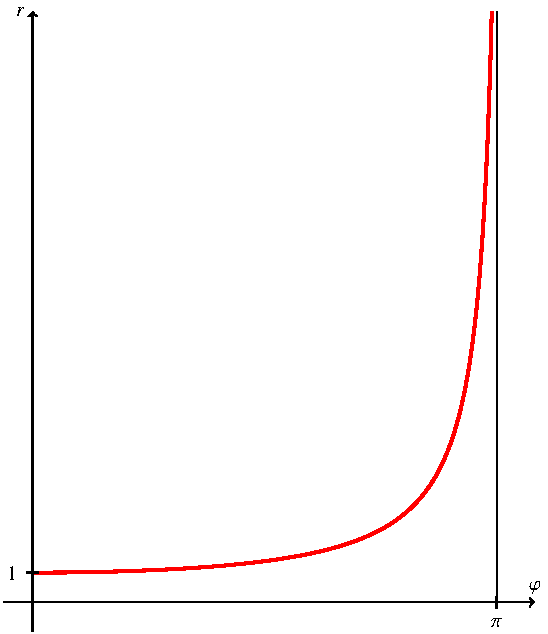
\includegraphics{chapters/tikz/lichtablenkung.pdf}
\caption{Die Lösung der Differentialgleichung~\eqref{skript:schwarzschild:udgl}
wächst in der Nähe des Ablenkungswinkels über alle Grenzen.
\label{skript:schwarzschild:abbildung:rphi}}
\end{figure}
Leider eignet sich die Differentialgleichung~\eqref{skript:schwarzschild:udgl}
nicht wirklich zur Berechnung des Ablenkungswinkels.
Schuld daran ist die Singularität, in der Nähe des Ablenkungswinkels
wächst $r(\varphi)$ über alle Grenzen, wie
Abbildung~\ref{skript:schwarzschild:abbildung:rphi} zeigt.

\subsection{Differentialgleichung für den Winkel}
Genau auf dem gleichen Weg wie wir eine Differentialgleichung für $r(\varphi)$
abgeleitet haben, können wir auch eine Differentialgleichung für
$\varphi$ als Funktion $r(\varphi)$ von $\varphi$ herleiten.
Dazu beachten wir, dass
\begin{align*}
\frac{d\varphi}{dr}&=\frac{\dot \varphi(s)}{\dot r(s)}
\qquad\text{und}
\\
\frac{d^2\varphi}{dr^2}
&=
\frac{\ddot\varphi(s)\dot r(s)-\ddot r(s)\dot\varphi(s)}{\dot r(s)^3}
\end{align*}
und setzen wie vorhin die bekannten Ableitungen $\ddot r(s)$ und
$\ddot\varphi(s)$ ein.
Wir erhalten
\begin{align*}
\frac{d^2\varphi}{dr^2}
&=
-\frac{2}{r}\frac{d\varphi}{dr}
-\frac{2r-3r_g}{2}\biggl(\frac{d\varphi}{dr}\biggr)^3
%\\
%&=
%-{{4\,\left({{d}\over{d\,s}}\,\varphi\left(s\right)\right)\,\left(
% {{d}\over{d\,s}}\,r\left(s\right)\right)^2+\left(2\,r^2\left(s
% \right)-3\,{\it rg}\,r\left(s\right)\right)\,\left({{d}\over{d\,s}}
% \,\varphi\left(s\right)\right)^3}\over{2\,r\left(s\right)\,\left({{d
% }\over{d\,s}}\,r\left(s\right)\right)^3}}
\end{align*}
Auch hier kann man mit $u=r/r_g$ wieder einen dimensionslosen Parameter
einführen, die Differentialgleichung vereinfacht sich dann zu
\begin{equation}
\frac{d^2\varphi}{du^2}
=
-\frac2{u}\frac{d\varphi}{du} -\frac{2u-3}2\biggl(\frac{d\varphi}{du}\biggr)^3.
\label{skript:schwarzschild:phidgl}
\end{equation}
Für diese Differentialgleichung ist es unproblematisch, die
Integration auch für grosse Werte von $u$ durchzuführen.

Die Differentialgleichungen
\eqref{skript:schwarzschild:udgl}
und
\eqref{skript:schwarzschild:phidgl}
können in Kombination dazu verwendet werden, den Ablenkungswinkel
numerisch zu berechnen.
Dazu verwendet man erst die Differentialgleichung
\eqref{skript:schwarzschild:udgl}
mit Anfangsbedingung
\begin{equation*}
\begin{aligned}
u(0)&=r/r_g,
\qquad&\qquad
u'(0)&=0.
\end{aligned}
\end{equation*}
bis zum $\varphi$-Wert $\varphi=\frac{\pi}4$.
Anschliessend kann man die
Differentialgleichung~\eqref{skript:schwarzschild:phidgl}
\begin{equation*}
\begin{aligned}
\varphi\biggl(u\biggl(\frac{\pi}2\biggr)\biggr)&=\frac{\pi}2,
\qquad&\qquad
\varphi'\biggl(u\biggl(\frac{\pi}2\biggr)\biggr)&=\frac1{u(\frac{\pi}2)}
\end{aligned}
\end{equation*}
bis zu einem sehr grossen Radius integrieren. 
Der Wert von $\varphi(u)$ strebt dabei gegen einen Wert
$\varphi_\infty>\frac{\pi}2$, der Ablenkungswinkel kann daraus als
\[
\alpha
=
(2\varphi_\infty - \pi)
\]
berechnet werden.
Das File \texttt{lichtablenkung.m} im Repository zeigt, wie dies mit
Octave gemacht werden kann.

